\documentclass[12pt,a4paper]{report}
\usepackage{amssymb,amsthm,amsmath,amscd}
\usepackage{latexsym}
\usepackage{enumerate}
\usepackage[german]{babel}
\usepackage{verbatim}
\usepackage[utf8]{inputenc}
\usepackage{hyperref}
\usepackage{graphicx}

%  theorem environments
\newtheorem{thm}{Satz}[section]
\newtheorem{cor}[thm]{Korollar}
\newtheorem{lem}[thm]{Lemma}
%\newtheorem{prop}[thm]{Proposition}
%\newtheorem{ax}{Axiom}

\theoremstyle{definition}
\newtheorem{defn}[thm]{Definition}
\newtheorem{rem}[thm]{Bemerkung}
\newtheorem{exa}[thm]{Beispiel}



\begin{document}
% ---------------

\begin{titlepage}
	\begin{center}
		
		\vspace*{1.0cm}
		\huge
		\textsc{\bf{PS Netze und Verteilte Systeme}}
		
		\vspace*{4.0cm}
		\textsc{
			\normalsize{eingereicht von} \\[0.5\baselineskip]
			{\large Baumgartner Dominik}
		}
		
		\vspace*{3.0cm}
		\textsc{
			\normalsize{Gruppe 1(13:00)}
		}
		
	\end{center}
	
\end{titlepage}


\textbf{Aufgabe 5:}
\\
\\
Wer war Guglielmo Marconi und was hat er/sie mit „Netzen“ zu tun? Recherchieren Sie über
Wikipedia hinaus und geben Sie alle Quellen an!\\
\\
Geboren am 25.04.1874 in Italien. War Pionier der drahtlosen Kommunikation.
Gründete 1897 Firma: The Wireless Telegraph \& Signal Company Limited.
Patentierte 1902 ein Gerät zum aufspüren magnetischer Signale sog. wireless Reciever. Erhielt 1909 Nobelpreis in Physik
Quellen:\\
\\
\url{http://www.nobelprize.org/nobel_prizes/physics/laureates/1909/marconi-bio.html}\\
\\
\\
\textbf{Aufgabe 6:}
\\
\\
Ein Protokoll-Stack habe eine $n$-schichtige Hierarchie. Die Applikationen erzeugen Nachrichten
von $M$ Byte Länge. Auf jeder Schicht wird ein h Byte großer Header hinzugefügt. Welcher Teil der
Netzwerk-“Bandbreite“ wird für die Nutzdaten verwendet? Was ist der Overhead? Diskutieren Sie
das Ergebnis im Hinblick auf die Anzahl der Schichten $n$, Größe der Header $h$ und Größe der
Nachrichten $M$.\\
\\
Anz. Schichten: $n$\\
Größe header pro Schicht: $h$\\
Größe der Nachricht. $M$\\
\\
Gesamtgröße der Übertragung:
\[
g=M+h\cdot n
\]
Nutzung zu Gesamtröße:
\[
\frac{M}{g}=\frac{M}{M+h\cdot n}= \frac{1}{1+\frac{h\cdot n}{M}}
\]
Je mehr Layer \& je größer jeder header, desto weniger Bandbreite wird für d. Nutznachricht verwendet.
\newpage
\textbf{Aufgabe 7:}
\\
\\
Was unterscheidet „Packet switching", „Circuit switching" und „Message switching“? Erkläre anhand von passenden Beispielen.
\\
\begin{itemize}
\item Circuit switching:\\
Verbindung zw. Sender \& Empfänger aufgebaut $\rightarrow$ Exklusiv für Nachrichten zw. Sender \& Empfänger reserviert. z.B. klassisches Telefonnetz.
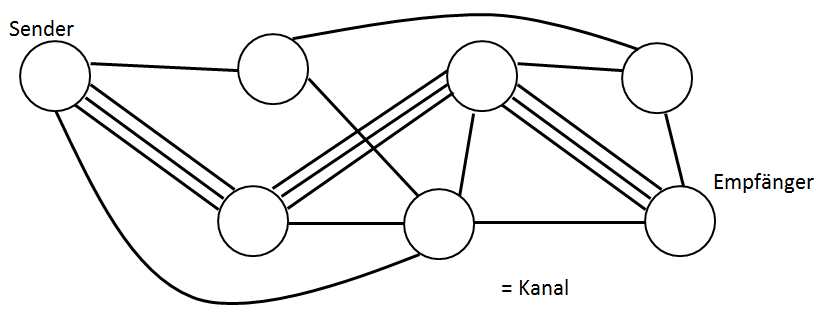
\includegraphics[scale=0.8]{7-1.png}
\\
\item Message switching:\\
Nachricht als Ganzes Verbindungslos vom Sender zum Empfänger weiter gereicht. Immer wieder in Zwischenstationen zwischengespeichert und dann weitergesendet. Immer gesamte Nachricht weitergesendet. z.B. E-Mail\\
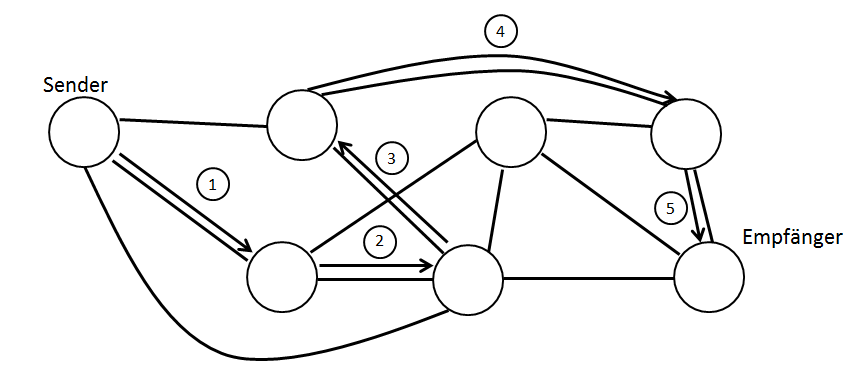
\includegraphics[scale=0.8]{7-2.png}
\\
\item Packet switching: Nachricht in Pakete aufgeteilt. Jedes Paket wird vom sender zum Empfänger weitergeleitet. z.B. UMTS\\
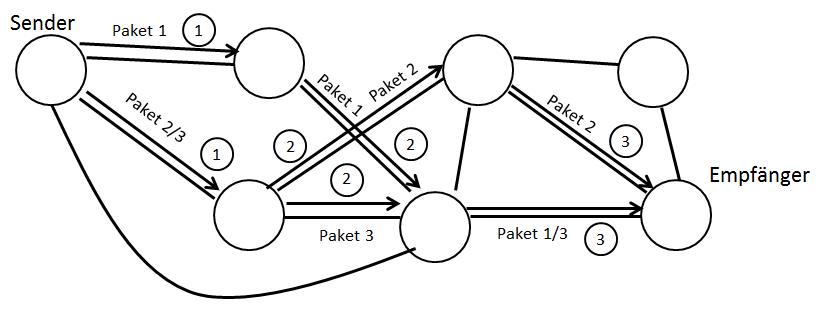
\includegraphics[scale=0.8]{7-3.png}
\end{itemize}
\newpage
\textbf{Aufgabe 8:}
\\
\\
Geben Sie die Bit-Folge wieder, die aus der Kodierung des Wortes ‘NVS2015’, gegeben in UTF-16BE Code-Points (ohne Byte Order Mark), mit Manchester-Kodierung resultiert.
\\
\\
UTF16:\\
Zahlen: 48-57\\
Großbuchstaben: 65-90\\
Kleinbuchstaben: 97-122\\
\\
Code:\\
\begin{tabular}{c c}
	0000000001001110 & 0000000001010110\\
	0000000001010011 & 0000000000110010\\
	0000000000110000 & 0000000000110001\\
	0000000000110101
\end{tabular}\\
\\
Manchester Code: Jedes bit als Flanke definiert
\begin{itemize}
	\item[-] 1 bit: teigende Flanke (von 0 nach 1)
	\item[-] 0 bit: fallende Flanke (von 1 nach 0)
\end{itemize}
(IEEE 802,3 Definition)\\
\\
Code:\\
\begin{tabular}{c c}
	10101010101010101001101001010110 & N\\
	10101010101010101001100110010110 & V\\
	10101010101010101001100110100101 & S\\
	10101010101010101010010110100110 & 2\\
	10101010101010101010010110101010 & 0\\
	10101010101010101010010110101001 & 1\\
	10101010101010101010010110011001 & 5\\
\end{tabular}\\
\newpage
\textbf{Aufgabe 9:}
\\
\\
Aufgabenstellung wie 8), es ist jedoch ein 4B5B Code und dann ein MLT-3 (Ternary) Code,
wie etwa bei 100Base-TX verwendet, anstatt der Manchester-Kodierung anzuwenden
(Spannungspegel: +, 0, -. DC-Balance beachten - 0=Startpegel). Wozu wird der MLT-3 Code bei
100Base-TX verwendet und warum ist dies notwendig?
\\
\begin{itemize}
\item 4B5B:\\
Code:\\
\begin{tabular}{c c c c}
	11110 & 11110 & 01010 & 11100\\
	11110 & 11110 & 01011 & 01110\\
	11110 & 11110 & 01011 & 10101\\
	11110 & 11110 & 10101 & 10100\\
	11110 & 11110 & 10101 & 11110\\
	11110 & 11110 & 10101 & 01001\\
	11110 & 11110 & 10101 & 01011\\
\end{tabular}\\
\item MLT-3: Folge: [0,+,0,-]: bei 1 Signal weiter rotiert.\\
Code:\\
\begin{tabular}{c c c c}
	+0-00 & +0-00 & 0++00 & -0+++\\
	0-0++ & 0-0++ & +00-0 & 0+0--\\
	0+0-- & 0+0-- & -00+0 & --00+\\
	0-0++ & 0-0++ & 00--0 & ++000\\
	-0+00 & -0+00 & --00+ & 0-0++\\
	0-0++ & 0-0++ & 00--0 & 0+++0\\
	-0+00 & -0+00 & --00+ & +00-0\\
\end{tabular}\\
\item MLT-3 verwendet um Erhöhung d. Taktfrequenz zu vermeiden / mehr Info in 1 Takt zu übertragen.
\item Nachricht vergrößert sich wegen 4B5B.Codierung um 25\%; um gleiche Übertragunsgeschw. für Nuterdaten beizubehalten, müsste diese auf 125 Mbit/s erhöht werden. Um dies bei gleicher Codierung mit 2 Zuständen zu erreichen, müsste die Übertragungsfrequenz erhöht wreden $\rightarrow$ will man aber nicht; stattdessen weiteren Zustand einführen $\Rightarrow$ mit 1 Takt können 4 bit übertragen werden.
\\
\\
\begin{tabular}{c | c}
	Vor MLT-3: & Nach MLT-3:\\
	$W=\frac{C}{2\cdot \log_2M=}=\frac{100\frac{Mbit}{s}}{2\cdot \log_2(2)bit}=$50MHz & $W=\frac{125\frac{Mbit}{s}}{2\cdot \log_2(4)bit}$=31,25MHz
\end{tabular}\\
\end{itemize}

















\textbf{Aufgabe 10:}
\\
\\
Skizzieren Sie die Funktionsweise des Kanalzugriffs-Schemas CSMA/CD und erklären Sie die
folgenden Begriffe: (a) Carrier Sense (b) Binary Exponential Back-off (c) Jam Sequence
\\
\\
CSMA (\textbf{C}arrier \textbf{S}ense \textbf{M}ultiple \textbf{A}ccess)/CD (\textbf{C}ollision \textbf{D}etection)
Bei Konflikt Sendeabbruch, mit Verzögerung erneut gesendet.
\begin{itemize}
\item[(a)] \textbf{Carrier Sense:}
Mehrere Teilnehmer verwenden das gleiche Medium zur Datenübertragung. Carrier Sense bedeutet, dass jeder Teilnehmer nur sendet, wenn das Medium frei ist, also wenn kein anderer Teilnehmer sendet.
3 existierende Arten:\\
1-persistent: wenn frei  senden.\\
p-persistent: mit Wahrscheinlichkeit von p gesendet wenn frei.\\
non-persistent: wenn besetzt  zufällige Zeit gewartet, wenn dann frei  senden.

\item[(b)] \textbf{Binary Exponential Back-Off:}
Wird eine Kollision erkannt, wird das Senden beendet. Neuer Sendeversuch noch 0 oder einer Slot-time ($2^1$ Möglichkeiten). Eventuell wieder Kollision  0,1,2,3 Slot-times Wartezeit ($2^2$ Möglichk.). Evtl. wieder Kollision $\rightarrow 2^3$ Mgl. Wartezeiten.\\
$\Rightarrow$ "binary-exponential". Nach 16 erfolglosen Versuchen folgt Abbruch.

\item[(c)] \textbf{Jam Sequence:}
Wird von einem sendenden Teilnehmer eine Kollision festgestellt, stellt dieser das Senden von Daten ein und sendet Jam Sequenz um anderen Teilnehmern mitzuteilen, dass eine Kollision stattgefunden hat. die Jam Sequence stellt sicher, dass die Kollision solange anhält, damit alle Teilnehmer diese erkennen können.
\end{itemize}





% -------------
\end{document}
